\chapter{Synthetic Nervous System Simulation}\label{ch:sns}
\graphicspath{{figs/60-sns/}{figs/60-sns/AnimatLab_reference/}}

The actuator and torque models of Chapters~\ref{ch:muscles} and~\ref{ch:torque} describe the robot's mechanics. Studying their interaction with neural control also requires a simulation that connects the mechanical model to a synthetic nervous system (SNS). I first attempted this integration in AnimatLab by combining a published walker with a spinal controller. The model produced stepping-like motion in air, but hand tuning did not produce walking. This chapter explains how that attempt motivated the development of software tools for assembling, testing, and comparing neuromechanical models.

\section{The AnimatLab Bipedal Walker}\label{sec:prior_walker}

For a course project in ME 610: Neuromechanical Modeling, Morrow and I combined the bipedal mechanics of \citet{li_bipedal_2017} with the two-level central pattern generator (CPG) of \citet{deng_neuromechanical_2019} in AnimatLab \citep{cofer_animatlab_2010}. The mechanical model had a pelvis and bilateral thigh, shank, foot, and toe segments, with sagittal-plane joints and antagonist Hill-type muscles at the hip, knee, and ankle. I added a passive toe joint. The initial controller used one rhythm generator (RG) to control both sides, with a separate pattern-formation layer. I added afferent feedback and heel- and toe-contact signals during the subsequent development. Figure~\ref{fig:animatlab_model_architecture} shows the model and controller organization.

I adjusted applied currents, synaptic weights, and muscle parameters by hand. The suspended model developed alternating muscle activity and stepping-like motion, presented at the 2021 NIH BRAIN Initiative Investigators Meeting \citep{bolenTorqueValuesArtificialKnee2021June15-17}. It did not achieve weight-bearing walking. This suspended stepping result preceded the later feedback and bilateral-RG extensions; it does not demonstrate walking with those additions.

I subsequently expanded the neural model into left- and right-side circuits with interconnected rhythm generators (RGs). I constructed the right-side subsystems from the left-side organization and linked the two RGs through commissural pathways. This later model is referred to as the Walker Two-Layer (W2L) model. Further circuit schematics and implementation records are provided in Appendix~\ref{app:simulation_verification}.

The AnimatLab result established that the combined model could produce stepping-like motion under suspension, but it did not establish weight-bearing walking. It also left unanswered how the controller would behave with the human musculotendon mechanics or BPA routing used elsewhere in this project. Investigating those questions required a way to connect the circuit to each mechanical model, inspect its signals, and test the connections before interpreting whole-model behavior.

\begin{figure}[p]
\centering
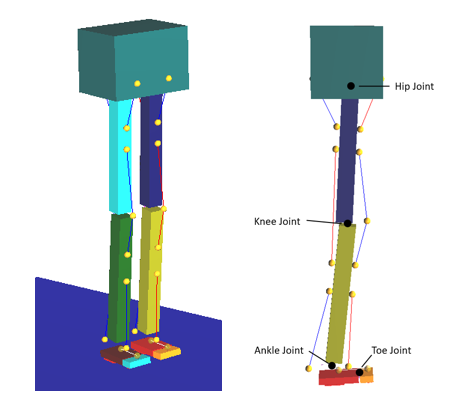
\includegraphics[width=0.64\textwidth,height=0.30\textheight,keepaspectratio]{OurWalker.png}
\par\medskip
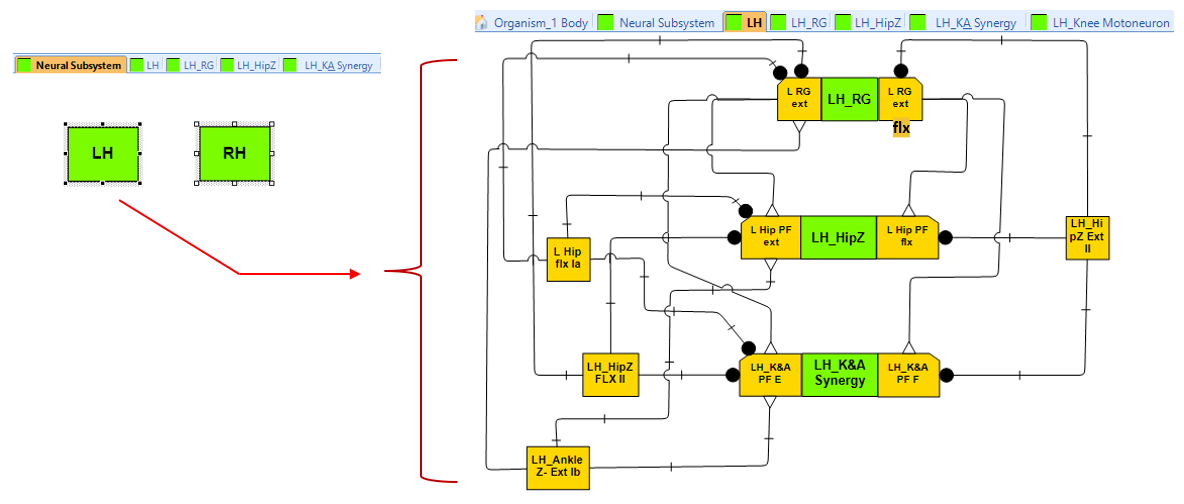
\includegraphics[width=\textwidth,height=0.31\textheight,keepaspectratio]{2layerImprove.png}
\caption[AnimatLab walker and controller hierarchy]{AnimatLab walker (top) and bilateral controller hierarchy (bottom). The model combines the Li walker mechanics and Deng CPG organization. These diagrams show construction; the suspended stepping result is described in the text.}
\label{fig:animatlab_model_architecture}
\end{figure}

\section{Knowledge Gaps and the New Tools}\label{sec:sns_gaps}

I developed tools for connecting neural controllers to the mechanical models used in this project. The work addressed five integration tasks:
\begin{enumerate}
    \item Convert the Gait2392 human model from OpenSim to MuJoCo and connect it to an SNS-Toolbox CPG controller.
    \item Couple a BPA-routed robot counterpart to a CPG controller so that artificial-actuator mechanics can be examined.
    \item Combine the Li walker mechanics, Deng neural organization, and foot-contact feedback, and test the resulting controller and mechanical interfaces.
    \item Construct neural circuits graphically in Simulink and connect them to mechanical simulations.
    \item Bring SolidWorks-derived mechanisms and MATLAB BPA models into the same development workflow as the neural controller.
\end{enumerate}
These tasks have different completion levels. The converted models, actuator-force calculation, graphical neural blocks, and selected interface tests are described below. Importing a mechanism or reproducing a rhythm does not establish that a complete coupled model walks. Table~\ref{tab:sns_capability} summarizes each gap, why it mattered, the tool built, and the outcome that demonstrates it.

Existing software supplied separate parts of the solution. OpenSim supplied musculoskeletal geometry, MyoConverter translated it to MuJoCo, and SNS-Toolbox supplied neuron and synapse models \citep{delp_opensim_2007, caggiano_myosuite_2022, todorov_mujoco_2012, nourse_sns_2023}. The MuJoCo version used here supports scripted simulation and parameter searches but uses rigid tendons; its Python interface does not provide the block-based circuit assembly needed for this workflow. Simulink supplies that graphical construction, while Simscape Multibody imports mechanical geometry, including SolidWorks-derived mechanisms. AnimatLab retains the reference controllers but is unsupported, relies on an older physics engine, and ran these simulations slowly. The tools connect these complementary environments and use matched tests to check what transfers between them.

\section{Software Tools}\label{sec:preliminary_sim_methods}

The tools connect musculoskeletal geometry, actuator forces, and neural circuits. Table~\ref{tab:sns_capability} summarizes the integration gaps and the tools that closed them. Figure~\ref{fig:pipeline} shows their relationship to the proposed hardware system.

\begin{table}[htbp]
\caption[Integration gaps and the tools that closed them]{Each integration gap this project faced, why it mattered, the tool developed, and the outcome that demonstrates the tool. The five rows correspond to the five tasks of Section~\ref{sec:sns_gaps}.}
\label{tab:sns_capability}
\small
\begin{tabularx}{\textwidth}{@{}>{\raggedright\arraybackslash}p{0.22\textwidth}>{\raggedright\arraybackslash}p{0.24\textwidth}>{\raggedright\arraybackslash}p{0.24\textwidth}>{\raggedright\arraybackslash}X@{}}
\toprule
\textbf{Integration gap} & \textbf{Why it mattered} & \textbf{Tool developed} & \textbf{Demonstrated outcome} \\
\midrule
No SNS control of these musculoskeletal models in a maintained engine & Scriptable simulation and parameter search require a modern engine with a Python interface & OpenSim-to-MuJoCo conversion with muscle-path and contact repair procedures, coupled to SNS-Toolbox & Conversion checks passed (paths, torque directions, frames, contact); closed-loop supported stepping with perturbation robustness (Section~\ref{sec:w2l_perturbation}) \\
No neuromechanical loop driven by BPA force & Artificial-actuator mechanics can only be examined with the real force law inside the loop & Actuator-force calculation: simulated length and pressure in, Festo-model force out, applied along the simulated route & The BPA-routed robot model air-steps and stands within the \qty{620}{\kPa} ceiling \\
The contact-driven Li--Deng walker existed only in an unsupported engine & Its control principles could not be tuned or extended reproducibly & W2L port to MuJoCo with the corrected connectome, per-synapse conductance solve, and weight-support harness & Cross-engine rhythm agreement; harness support weaned 70 to 10 percent with re-tuning; robust to $\pm 20$ percent segment-mass mismatch at frozen conductances \\
No graphical circuit construction against real mechanics & Circuits had to be hand-coded, blocking lab-wide use & SNS-Simscape block library wired to mechanical simulation & Reflex demonstrations and matched-circuit comparisons (periods matched at \qty{1.000}{\second}, correlation at least 0.99996) \\
CAD mechanisms and BPA models lived outside the neural workflow & The design loop was fragmented across incompatible tools & SolidWorks and OpenSim mechanism imports with the MATLAB BPA models in one workflow & Mechanism import achieved alongside the neural and actuation tools \\
\bottomrule
\end{tabularx}
\end{table}

\subsection{Model Conversion and Actuator Coupling}\label{sec:sns_existing_tools}

MyoConverter supplies the initial OpenSim-to-MuJoCo translation, and the conversion checks that accompanied it found and corrected five concrete problems. My first attempt converted the robot model itself, in which the braided-pneumatic routing had been laid over the human Gait2392 skeleton with the human muscle parameters left unchanged, and MyoConverter's equilibrium checks flagged the combination as infeasible because the routed path lengths depart far from the lengths those parameters describe. The workable sequence converted the unmodified human reference model first, then regenerated the robot routing on both legs through a mirroring procedure that also restored muscles disabled by earlier test configurations. Three very small hip rotators per side, the quadratus femoris, gemelli, and piriformis, are poorly conditioned even in OpenSim, and I rendered their actuators inert at model load, so the converted model keeps its 92 muscle-tendon actuators with six of them carrying no force. MuJoCo's default axis convention differs from the OpenSim and International Society of Biomechanics convention, and the converted model keeps the OpenSim convention: the axis remap is embedded in the body frames, joint values transfer unchanged, and only externally applied vectors such as ground-reaction forces require an explicit remap, which a pose-translation probe verified. The source model defines the patella through vastii insertion locations that move with knee angle rather than through a coordinate transform, and the converter realizes those moving insertions as coupled follower joints whose sampled range limits conflicted with the coupling constraints until the limits were removed; the rectus femoris route, which lacks the patella tracking, was rerouted over the vastii tracking point. Ground contact initially dragged on an invisible floor because the converted collision pairs ignore the per-geometry contact flags, and restricting contact to the six foot--ground pairs, with passive torques replacing the joint stops that the conversion dropped, removed the artifact. Comparing attachment paths with the OpenSim source checked the transferred geometry, and activating individual actuators checked the direction of the resulting joint torque. These checks concern conversion fidelity, not the ability of the controller to produce walking. The neural and mechanical models exchange signals at a \qty{2}{\milli\second} step.

For the BPA-routed robot model, an actuator-force calculation connects the neural and mechanical simulations. It takes the simulated muscle length and pressure as inputs and evaluates the quasi-static force model from Chapter~\ref{ch:muscles}; the resulting force acts along the simulated actuator path. This calculation does not include valve or pressure dynamics. Length, velocity, force, and foot-contact signals return to the controller through sensory channels. The correction terms of Chapter~\ref{ch:torque} do not by themselves establish that transferred routing and compliance are correct in a dynamic model; those properties require separate checks.

\subsection{Graphical Circuit Construction}\label{sec:sns_new_tools}

The SNS-Simscape library implements neuron, synapse, afferent-encoder, activation, and muscle-force elements as editable Simulink blocks. The library retains the conductance-based neuron and synapse formulation supplied by SNS-Toolbox; it does not introduce a new neuron model. Verification uses selected circuits under matched inputs. Figure~\ref{fig:simulink_sns_implementation} shows the core blocks and graded-neuron signal flow.

OpenSim-derived and SolidWorks-derived mechanisms were imported into Simscape Multibody. These mechanical imports are separate from the standalone reflex demonstrations.

\begin{figure}[htbp]
\centering
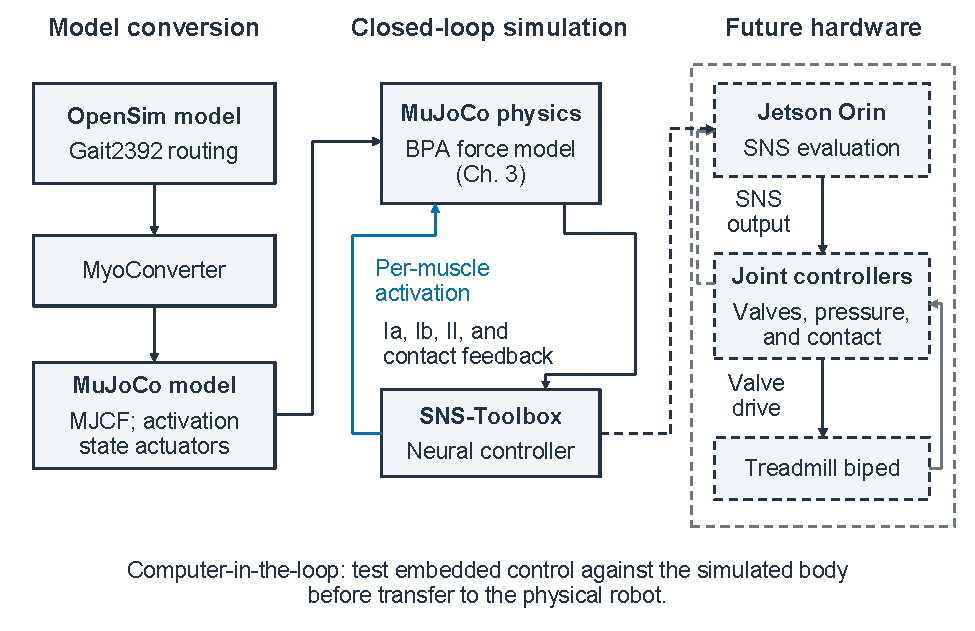
\includegraphics[width=\textwidth]{pipeline.pdf}
\caption[Simulation-to-robot pipeline]{Model conversion, closed-loop simulation, and proposed hardware deployment. Solid simulation interfaces connect neural activation to BPA force and return afferent signals. The embedded valve-control and network-evaluation system is future work (Chapter~\ref{ch:futurework}).}
\label{fig:pipeline}
\end{figure}

\begin{figure}[p]
\centering
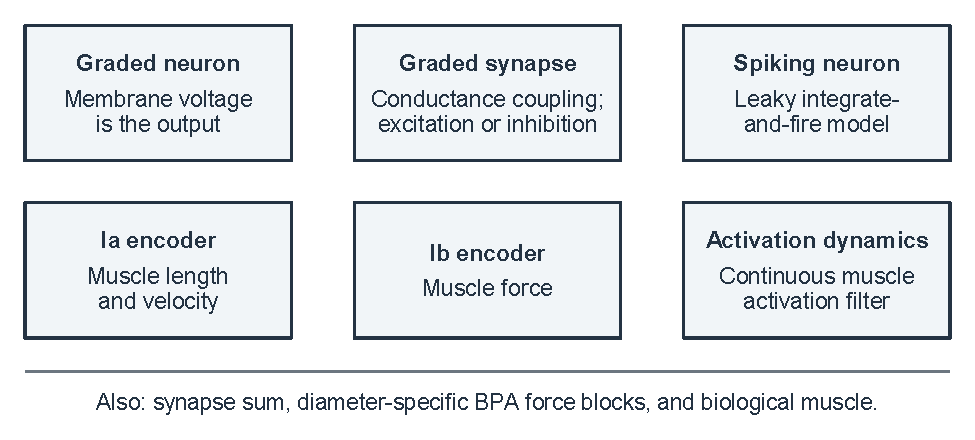
\includegraphics[width=0.94\textwidth,height=0.42\textheight,keepaspectratio]{sns_library_overview.pdf}
\par\medskip
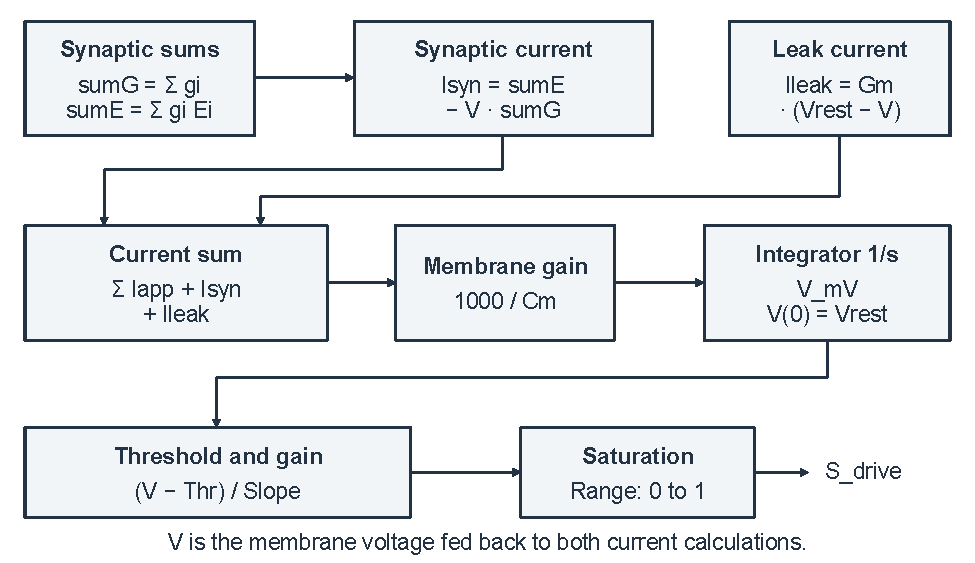
\includegraphics[width=0.94\textwidth]{simulink_neuron_detail.pdf}
\caption[Simulink SNS library blocks and neuron implementation]{Core SNS-Simscape blocks (top) and graded-neuron implementation (bottom). Summed currents drive membrane integration; threshold, inverse-slope gain, and saturation bound the output. Voltage feeds both current calculations. The generic BPA demonstration remains provisional.}
\label{fig:simulink_sns_implementation}
\end{figure}

\section{Verification of the Implemented Interfaces}\label{sec:preliminary_sim_results}

The tests address three distinct questions: whether a circuit produces its expected response, whether implementations agree under matched inputs, and whether the neural and mechanical models exchange signals in a closed loop.  The larger evaluation sets and their limitations are collected in Appendix~\ref{app:simulation_verification}; neuron equations and calibration details remain in Appendix~\ref{app:neuron_equations}.

\subsection{Reflex Response}\label{sec:sns_simulink_demos}

The library assembles Ia stretch excitation, reciprocal inhibition, and Ib autogenic inhibition in a reduced-order antagonist knee model (Figure~\ref{fig:simulink_reflex_topology}). A second demonstration tests the stretch reflex in an arm holding a beverage container as it is loaded. With the reflex enabled, arm sag was \ang{2.00}, compared with \ang{7.85} when it was disabled. The comparison checks the implemented feedback response; experimental calibration of the mechanical parameters remains necessary.

\begin{figure}[p]
\centering
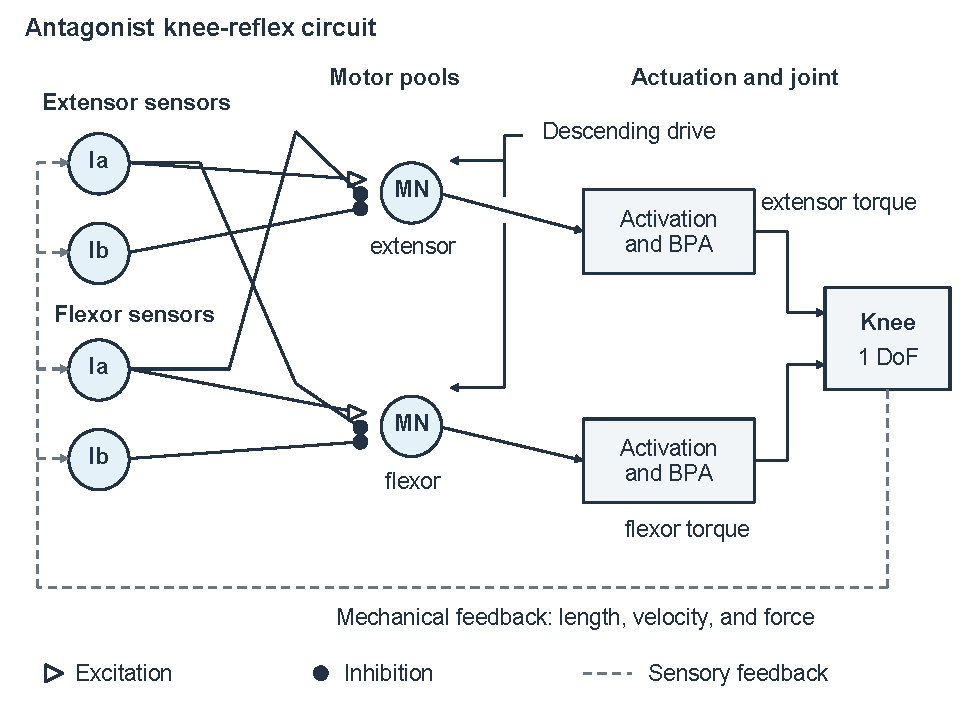
\includegraphics[width=\textwidth]{KneeReflex_circuit.pdf}
\caption[Reduced-order knee-reflex circuit topology]{Reduced-order antagonist knee-reflex circuit. Triangles mark excitation, and filled circles mark inhibition. Ia input excites the homonymous motor pool and inhibits its antagonist; Ib input inhibits the homonymous pool. Motor output drives activation and BPA-force blocks. Mechanical parameters and the generic BPA block remain provisional.}
\label{fig:simulink_reflex_topology}
\end{figure}

\subsection{Matched Neural Implementations}\label{sec:crossengine_results}

The contact-driven W2L rhythm core was implemented in NumPy and native Simulink blocks from a common connectivity specification. Both implementations received the same input protocol. Burst periods matched at \qty{1.000}{\second}, all ten expected bursts were reproduced, and voltage-trace correlation was at least 0.99996 (Figure~\ref{fig:w2l_crossengine}). The agreement is specific to this circuit and input protocol.

Removing the phasic heel-contact inputs caused the circuit to latch in both implementations. The alternating activity therefore depends on the specified sensory drive.

\begin{figure}[htbp]
\centering
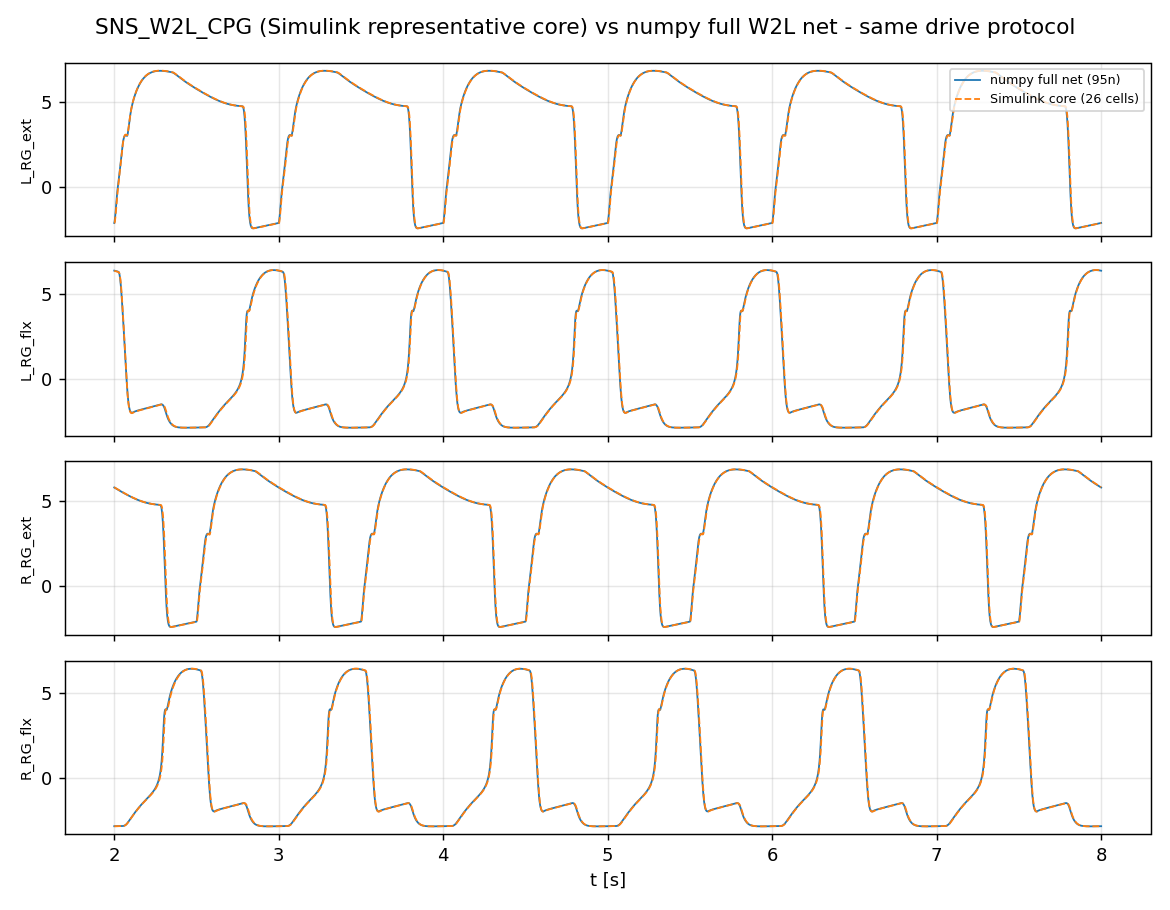
\includegraphics[width=\textwidth,height=0.55\textheight,keepaspectratio]{sns_w2l_traces.png}
\caption[W2L rhythm-core traces across engines]{W2L rhythm-generator voltages under matched inputs in NumPy and Simulink. Burst periods and counts agree; full-trace correlation is at least 0.99996. The residual \qty{2}{\milli\second} lag is one discrete solver step. The test concerns the driven rhythm core, not walking mechanics.}
\label{fig:w2l_crossengine}
\end{figure}

\subsection{Closed-Loop Model Coupling}

The MuJoCo--Simulink bridge, built on the official MathWorks blockset that embeds the MuJoCo model inside Simulink as the mechanical model, was tested against an independent Python integration using single-muscle activation, different control rates, and sensor readback. Readback was bit-exact over the scored window. The exported neural network also drove all 92 actuators during a \qty{5}{\second} open-loop run, without afferent return; the closed-loop reflex experiment exercised commands and sensory measurements through the same interface. However, under tonic drive alone the Simulink realization reached a fixed point while the NumPy reference oscillated. The network-level discrepancy remains a limit on transferring tuned controller parameters between implementations.

\subsection{Perturbation Robustness and Pathway Deletions}\label{sec:w2l_perturbation}

I tested the coupled W2L walker the way the perturbation literature tests neuromechanical models: the tuned conductances stay frozen, the perturbation is applied to the body or to the network, and recovery is judged from the gait itself (Figure~\ref{fig:w2l_perturbation}). Under a harness carrying \qty{25}{\percent} of body weight, the walker withstood every segment-mass change tested (thigh masses and distal-leg masses each scaled by $+10$, $-10$, $+20$, and $-20$ percent, and the whole leg by $\pm 10$ percent): ten of ten conditions, without a fall and with forward progression in each. An inhibitory tonic stimulus applied to the rhythm-generator layer for one second perturbed the rhythm without a fall, and stepping persisted through and after the stimulus window; a \qty{40}{\newton} fore-aft push at the pelvis likewise produced a transient excursion and recovery. Removing individual pathway classes then located the load-bearing connections. Deleting the Ia reciprocal chain, the Renshaw cells, the heel-contact cascade, or the crossed heel-to-contralateral-flexor edge left alternating stepping intact, whereas removing the commissural coupling reduced the gait to two strides and removing the Ib load feedback stopped stepping entirely. The same conductance set walks with the harness weight support re-tuned down a ladder from 70 to 10 percent of body weight, with a fresh-process verification at every step. These tests concern supported progression under the harness; unsupported walking is not established.

\begin{figure}[p]
\centering
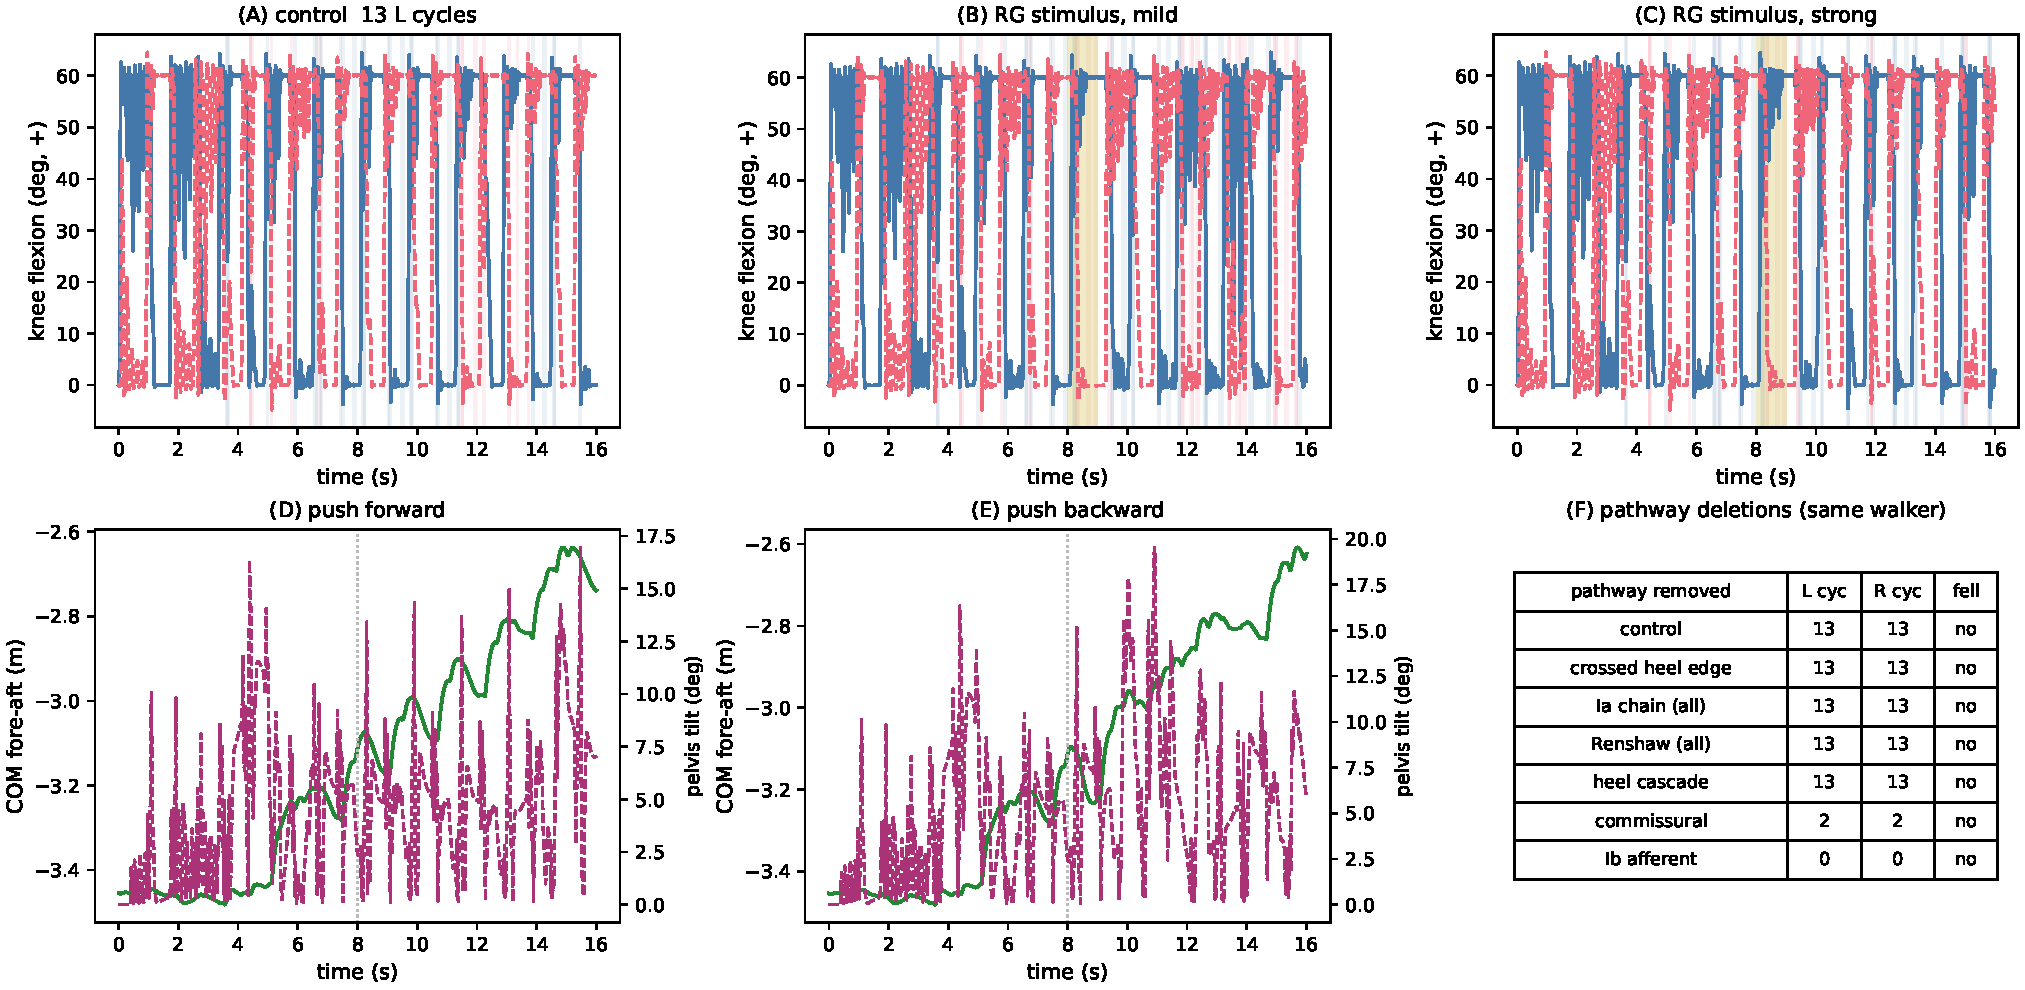
\includegraphics[width=\textwidth,height=0.52\textheight,keepaspectratio]{w2l_perturbation_panels.pdf}
\caption[W2L perturbation and pathway-deletion panels]{Perturbation tests of the corrected W2L walker in MuJoCo with all conductances frozen (harness at \qty{25}{\percent} weight support). (A--C) Left and right knee flexion (solid and dashed; heel contact shaded). (B, C) A one-second inhibitory tonic stimulus to the rhythm-generator layer (yellow band), mild and strong; stepping persists through and after the window. (D, E) Fore and aft \qty{40}{\newton} pelvis pushes at $t=\qty{8}{\second}$ (dotted line): fore-aft center-of-mass position (solid) and pelvis tilt (dashed). (F) Strides per leg when one pathway class is removed: most removals are compensated, while commissural coupling and Ib load feedback are load-bearing.}
\label{fig:w2l_perturbation}
\end{figure}

\section{Capabilities and Remaining Limits}\label{sec:sns_discussion}

The AnimatLab attempt motivated a repeatable way to connect neural circuits to mechanical models and test their individual interfaces. The resulting tools provide converted geometry, a BPA-force interface, graphical neural components, controller ports, and automated comparisons. The reflex and rhythm-core tests demonstrate specific circuit behaviors; the bridge tests demonstrate closed-loop signal exchange. Mechanical import, controller transfer, and locomotion performance remain separate validation problems.

The supported robot evaluations produced stepping-like motion and, in some configurations, forward progression, but no harness-free walking. Reducing tonic neural drive did not remove mechanical support. Spiking-neuron comparisons preserved a continuous motor-activation interface while changing rhythm timing and, in some runs, limb coordination (Appendix~\ref{app:simulation_verification}).

The next step is to use these interfaces and tests to improve weight-bearing control and then evaluate transfer to hardware. Chapter~\ref{ch:futurework} discusses those extensions. 
